%----------------------------------------------------------------------------------------
%	PACKAGES AND OTHER DOCUMENT CONFIGURATIONS
%----------------------------------------------------------------------------------------
\documentclass[a4paper,11pt]{article}
\usepackage[a4paper,textwidth=140mm,textheight=245mm]{geometry}
\usepackage[utf8]{inputenc}
\usepackage{listings}
\usepackage{graphicx}
\usepackage{float}
\usepackage{mathtools}
\usepackage{multicol}
\usepackage{caption}
\makeatletter
\renewcommand{\section}{\@startsection
   {section}%                         name
   {1}%                               level
   {0mm}%                             indent
   {-1.5\baselineskip}%               space above header
   {0.5\baselineskip}%                space under header
   {\sffamily\bfseries\upshape\normalsize}}% style
\renewcommand{\subsection}{\@startsection
   {subsection}%                      name
   {2}%                               level
   {0mm}%                             indent
   {-0.75\baselineskip}%              space above header
   {0.25\baselineskip}%               space under header
   {\rmfamily\normalfont\slshape\normalsize}}% style
\renewcommand{\subsubsection}{\@startsection
   {subsubsection}%                    name
   {3}%                               level
   {-10mm}%                             indent
   {-0.75\baselineskip}%              space above header
   {0.25\baselineskip}%               space under header
   {\rmfamily\normalfont\slshape\normalsize}}% style
\makeatother

\begin{document}

\begin{titlepage}
\title{TSBK07\\
Sammanfattning}
\author{Martin Söderén\\ marso329@student.liu.se\\900929-1098}
\date{\today}
\maketitle




\vfill % Fill the rest of the page with whitespace

\thispagestyle{empty}

\end{titlepage}

\section{level of detail}
\subsection{edge collapse}
A good edge is selected and the two vertices are replaced by one on the middle of the old edge. 
\subsection{vertex removal}
A good vertex is selected and one vertex connected to the first vertex by and edge is moved to the removed vertex. This can give undesirable shapes and neighbouring triangles can have very different size.skybox
\section{OpenGL built-in interpolation feature}
Simply refers to varying variables
\section{transformation chain}
model-to-world$\rightarrow$world-to-view$\rightarrow$projection$\rightarrow$device
\\
model-to-world: moves objectsin the world.\\
world-to-view : moves the camera\\
projection: changes the lens\\
viewport: resizes the window\\
\section{matrices}
\subsection{rotation around an arbitrary axis}
We want to rotate an object around an axis defined by $p_1$ and $p_2$.
\\First translate the axis to go through origo: $T(-p_1)$.\\
Second align the axis with any base axis:\\
\begin{enumerate}
\item let say the vector between $p_1$ and $p_2$ is $u$ and $z'=u$.
\item lets assume $u$ is not parallel with $x$ and make $y'=u\times x$
\item then $x'=y'\times z'$
\item the rotation matrix is now $R= \begin{vmatrix} x'_x&x'_y&x'_z&0\\ y'_x&y'_y&y'_z&0\\z'_x&z'_y&z'_z&0\\0&0&0&1 \end{vmatrix}$
\end{enumerate}
third: Rotate around the axis z.\\
fourth: undo $R$ which is $R^t$\\
fifth: undo the translation which is $T(p_1)$\\
the complete transformation is:
$$T(p_1)*R^t*R_z(\sigma)*R*T(-p_1)$$

\subsection{homogeneous coordinates}
By using homogeneous coordinates we can do addition by multiplications which is efficient for models with a lot of points. for example translation::

\begin{table}[H]
$$ \begin{vmatrix} 1&0&v_x\\ 0&1&v_y\\0&0&1 \end{vmatrix}*\begin{vmatrix}p_x\\p_y\\1 \end{vmatrix}=\begin{vmatrix}p_x+v_x\\p_y+v_x\\1 \end{vmatrix}$$
  \caption{Arbitrary axis shearing}
\end{table}


\subsection{Shearing}
\begin{itemize}
\item translate to origo
\item change of basis
\end{itemize}
\begin{table}[H]
$$ \begin{vmatrix} 1&s_x^y&s_x^z&0\\ s_y^x&1&s_y^z&0\\s_z^x&s_z^y&1&0\\0&0&0&1 \end{vmatrix}$$
  \caption{Arbitrary axis shearing}
\end{table}
This results in:
$$x'=s_x^y*y+s_x^z*z$$
$$y'=s_y^x*x+s_y^z*z$$
$$z'=s_z^x*x+s_z^y*y$$

\subsection{rotation}
Easiest way to remember all is to remember X and for Y all sinuses is moved one step to the right and down in a 3x3 matrix and if a sinus gets outside the 3x3 matrix it is transferred to the other side. 
\begin{table}[H]
$$ \begin{vmatrix} 1&0&0&0\\ 0&cos(phi)&-sin(phi)&0\\0&sin(phi)&cos(phi)&0\\0&0&0&1 \end{vmatrix}$$
  \caption{X rotation}
\end{table}

\begin{table}[H]
$$ \begin{vmatrix} cos(phi)&0&sin(phi)&0\\ 0&1&0&0\\-sin(phi)&0&cos(phi)&0\\0&0&0&1 \end{vmatrix}$$
  \caption{Y rotation}
\end{table}

\begin{table}[H]
$$ \begin{vmatrix} cos(phi)&-sin(phi)&0&0\\ sin(phi)&cos(phi)&0&0\\0&0&1&0\\0&0&0&1 \end{vmatrix}$$
  \caption{Z rotation}
\end{table}


\subsection{Translation}

\begin{table}[H]
$$ \begin{vmatrix} 1&0&0&X\\ 0&1&0&Y\\0&0&1&X\\0&0&0&W \end{vmatrix}$$
  \caption{Z rotation}
\end{table}

\subsection{Scaling}
\begin{table}[H]
$$ \begin{vmatrix} X&0&0&0\\ 0&Y&0&0\\0&0&Z&0\\0&0&0&W \end{vmatrix}$$
  \caption{Z rotation}
\end{table}

\subsection{normal matrix}
the normal matrix is the transpose inverse of the modelview matrix(if you dont have scaling).

\section{vectors}
\subsection{mirroring}
To mirror vector l in vector n. The mirror vector is $2l_n-l$ where $l_n$ is l normalized.
\section{lightning}
\subsection{radiosity}
Using form factors which describes how well patches can see each other light from light sources is bounced around between objects but the difference compared to ray casting is that each patch is considerer a light source that emits light.

\subsection{phong vs gouraud shading}
gouaraud is faster than phong. Gouraud can use the phong light model. Gouraud interpolates the shade over the surface and the result of the specular component can be bad if the polygon count is low. Gouraud is however very good for curved surfaces if the polygon count is high.\\
\\
In phong shading the normalvector of vertices is interpolated and each pixel is calculated with a unique normalvector. It renders surfaces even with low polygon count well. It support specular reflection. More computation heavy and the computation is done in the fragment shader once for each pixel.

\subsection{Phong shader}
$$i=k_di_a+\sum(k_di_smax(0,cos(\theta_s)+k_{spec}i_smax(0,cos(\theta_s)^n)$$
where:\\
$k_d$ is the diffuse constant for that element.\\
$i_a$ is the ambient light level\\
$i_s$ is the light intensity from the source\\
$\theta_s$ is the reflection angle between the source and the camera on the object.\\
$k_{spec} $ is the specular component of the object\\
$n$ is the shininess of the object

\subsection{jittering}
Varying the direction of a ray in ray-tracing. Used in anti-aliasing, when you look through glass which bends the image, When rendering fire which bends the light, out of focus effects, fuzzy reflection, soft shadows motion blur. Depth of field

\subsection{Shadows through ray-casting}
For each pixel you cast a ray from every light source and checks if it intersection any object between the light source and the current pixel. If it does that light source is not included in the calculation.
\subsection{Ray-casting}
The ray from the eye is the primary ray, the ray towards the light source is a shadow ray and a ray between objects is reflection ray.

\section{Skyboxes}
\begin{itemize}
\item Disable z buffering so it does not obscure anything
\item Center the skybox around the camera by removing the translation part of the world-to-view matrix
\item No lighting, because else it will look like a box
\item use GL\_CLAMP\_TO\_EDGE filtering for the textures
\end{itemize}

\section{Textures}
\subsection{Environment mapping}
Let say you have a mirror sphere which you want to reflect the environment. Then you surround it with some kind of bounding volume for example a cube. This could be a cubemap. For each pixel on the screen you cast a ray on the sphere and let it reflect on time towards the bounding volume. This can be done in the vertex shader and has low computational cost. 
\subsection{Problems with discontinuous coordinates}
Problem arises when a triangle exists over the texture  overlap so one vertex is below the overlap and the other two are above the overlap. This can be fixed by replacing that triangle with two new. or map that vertex to the correct value.
\subsection{Cylindrical mapping}
Cylindrical system:
$$x=R*cos(\theta)$$
$$y=R*sin(\theta) $$
$$z=z$$
for mapping this onto a texture we use:
$$u=arctan(y,x)$$
$$v=z$$
\subsection{Spherical mapping}
$$x=R*cos(\phi)*cos(\theta)$$
$$y=R*cos(\phi)*sin(\theta) $$
$$z=R*sin(\phi)$$
we want:
$$u=arctan(y,x)$$
$$v=sin^{-1}(z/R)$$

\section{Curve generation}
In a approximation spline the control points does not need to be on the line but in a interpolating spline they must lay on the line.  In a approximation spline the line must however reside in the convex hull of the control points.
\subsection{catmull-rum}
Is a interpolating spline which is defined by four control points and generates a spline between the two middle controlpoints. The next section is created by adding a new point and removing the first one.
\subsection{Bezier curve}
$C_0$ is no physical separation\\
$C_1:C_0$ and matching first derivatives\\
$C_2:c_1$ and matching second dericatives\\
$G_0=C_0$\\
$G_1$ and tangents points in the same direction\\
$G_2$ and the tangents are of the same length
$$p(u)=(1-u)^2p_0+2(1-u)up_1+u^2p2$$
How to show that $C_0$ and $G_0$ is fullfilled:\\
First segement is points 1,2,3 and the second is 4,5,6. Put these points in the equation so you get
$p(u)$ and $q(u)$ and make sure that that $p(1)=q(0)$. $C_1$ is fullfilled if $p'(1)=q'(0)$
\subsection{Quadratic bezier is interpolation of a interpolation}
Assume we have three control points $p_0$, $p_1$, $p_2$ and $p_3$. We create three new points in-between these points $r_0=p_0+(p_1-p_0)u$, $r_1=p_1+(p_2-p_1)u$ and $r_2=p_2+(p_3-p_2)u$. From these three we create two new points $s_0=r_0+(r_1-r_0)u$ and $s_1=r_1+(r_2-r_1)u$ and from these two we create a new point $t_0=s_0+(s_1+s_0)u$. By inserting these into each other you get $$p(u)=r_0(1-u)^2+r_12u(1-u)+r_2u^2$$ which is the quadratic bezier.
\subsection{Cubic bezier curves}
These can be seen as a linear combination of two quadratic bezier curves.
$$B(t)=(1-t)B_{P_0,p_1,P_2}(t)+tB_{P_1,p_2,P_3}(t), 0\leq t \leq 1$$
\section{Diamond square algorithm}
\begin{center}
\begin{figure}[H]
    \centering
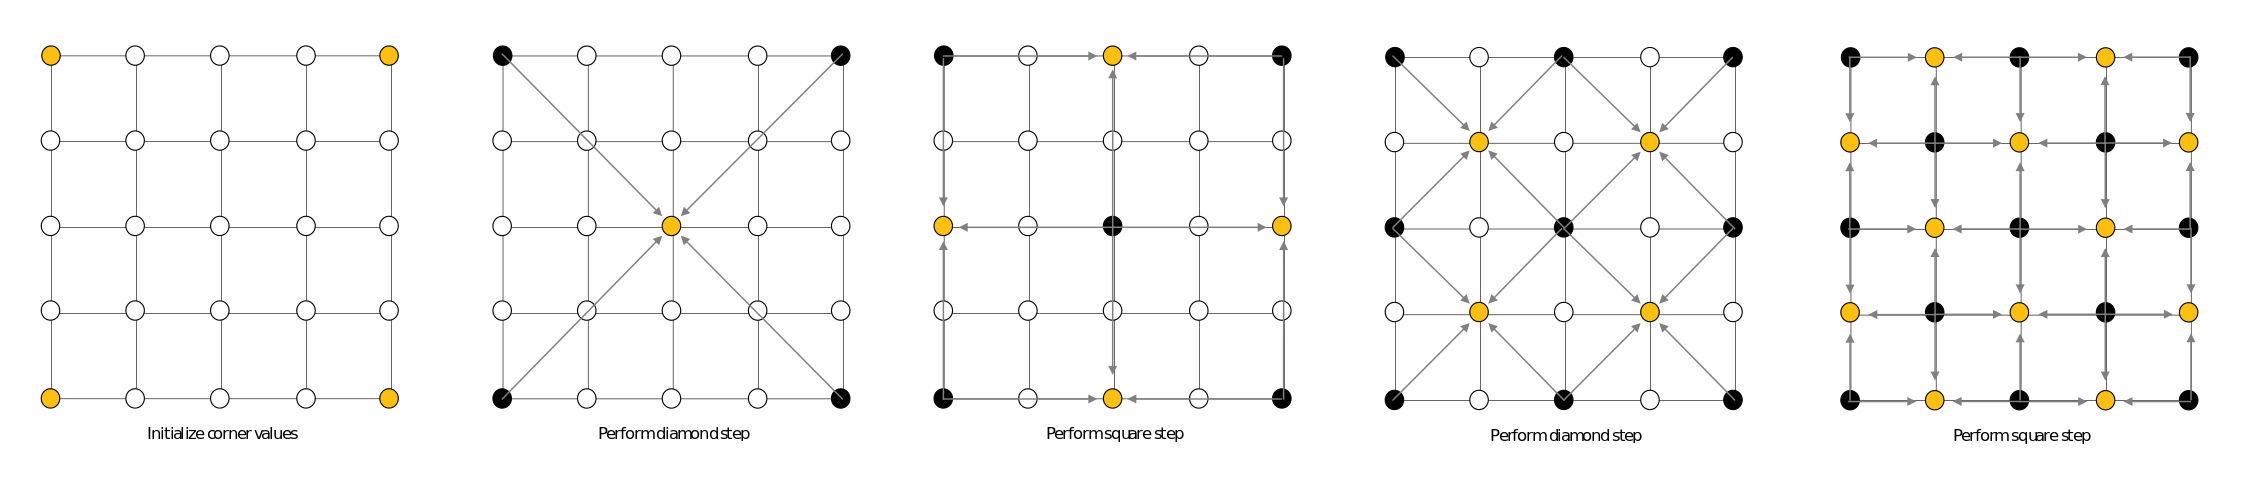
\includegraphics[scale=0.20]{diamond.png}
\caption{Diamond square}
\end{figure}
\end{center} 
\section{Bresenham line-drawing}
$p_0=2\Delta y-\Delta x$\\
$x_{n+1}=x_{n}+1$ \\
Om $P_n>0$ så är $P_{n+1}=P_n+2\Delta y-2\Delta x$ och $y_{n+1}=y_{0}+1$ \\
annars: $P_{n+1}=P_n+2\Delta y$ och $y_{n+1}=y_{0}$ \\

\section{3d effects in 2d}
Scaled sprites to give impression of depth. \\
Parallax scroll: The background moves more slowly than the object and the foreground moves faster.\\
Shadows can be implemented.

\section{Collision detection}
\subsection{Using SAT(Separating Axis
Theorem)}
For each plane in a object test for every vertex in the other object if that is inside
the other object by checking the difference between the dotproduct between the normals. This has to be done between object A and B but also between B and A

\section{anti-aliasing}
\subsection{supersampling}
renders the screen at a higher resolution anhd scales it down
\subsection{multisampling}
Renders some parts of the screen at a higher resolution and scales those down. 

\section{mipmap}
Mipmap does not help when there are different derivatives in different directions.\\
\\
GL\_texture\_mag\_filter:(the image is larger than the texture)always uses the largest mipmap\\
With this you can use either Gl\_nearest or gl\_linear.nearest takes the closest pixel and linear uses a average of the 4 closest pixels.\\
GL\_texture\_min\_filter(the image is smaller than the texture):\\
GL\_nearest:nearest pixel
gl\_linear: avera of the 4 closest pixels.\\
gl\_nearest\_mipmap\_nearest:nearest mipmap and nearest pixel \\
gl\_nearest\_mipmap\_linear:nearest mipmap and average pixel\\
gl\_linear\_mipmap\_nearest:so on\\
gl\_linear\_mipmap\_linear:so on\\
\section{gldrawarrays vs gldrawelements}
gldrawelements means less vertex shader computation but the fragment shader computation is the same. Also less data is sent with drawelements.
\section{Fractal}
\subsection{Self squaring fracals}
If you start outside the radius the function diverges immediately 
\\
julia set:
$$z_{k+1}=z_k^2+L$$
a algorithm for displaying a julia fractal image:
\begin{lstlisting}[language=c]
for y<maxy{
for x<maxy{
zr,zi=scaling of x,y
for i<maxiter{
z=z2+1;
if |z|>r break
}
draw(x,y)(different colors for different i)
}
}
\end{lstlisting}
 
\section{Frustum culling}
Used to minimized unnecessary rendering of objects which are not in eyesight of the user. You create a bounding sphere around each object. Each sphere has a location c and a radius r. You check each bounding sphere against each plane of the viewing frustum and check if $p=c+n.r$ which is the point on the sphere with the same normal as the frustum view plane(pointing inwards) and checks if this point is inside or outside the plane using the plane equation. If this fails for all planes then the object is outside the viewing frustum.

\section{back-face culling}
Is a part of the opengl pipeline and can be used to improve performance since it chooses not to render polygons that is facing away from the camera. This is decided for each polygon and the must be defined the same way clock-wise or counter-clock-wise. 

\section{Examples}
\subsection{Upload a float to vertex shader}
in opengl program:
\begin{lstlisting}
float time =clock_t();
glUniform1f(glGetUniformLocation(program, "time"),time);
\end{lstlisting}
In vertex shader:
\begin{lstlisting}
uniform float time;
\end{lstlisting}

\subsection{2tan}
$$atan2(x,y)=2arctan(\dfrac{y}{\sqrt{x^2+y^2}+x})$$ if $x>0 $ or $ y\neq0$ else $atan2(x,y)=\pi$
\end{document}

